\section{Related Works}
\label{sec:related_works}
\subsection{fMRI to Image Reconstruction}
Recent methods for fMRI to image reconstruction leverage pretrained CLIP and SDXL models to predict image features. Notably, MindEye \cite{scotti2023reconstructingmindseyefmritoimage} predicts CLIP embeddings from fMRI and uses diffusion based image generation to reconstruct seen images, while Brain-Diffuser \cite{ozcelik2023brain} combines visual representations with latent diffusion. MindEye2 further improves reconstruction through a shared-subject training and predicts OpenCLIP ViT/14 representations \cite{schuhmann2022laionb, ilharco_gabriel_2021_5143773} to be used for SDXL based image generation. These approaches demonstrate the value of pretrained visual representations and generative models from fMRI to image reconstruction. However, most of these approaches primarily operate on voxels or regions of interest (ROI) based neural representations rather than cortical flatmaps. Our work instead investigates whether flatmap representations can provide a suitable input for modern vision architectures.

\subsection{fMRI Representations}
The representations of fMRI activity are a central consideration in developing generalizable neural representations. Traditional approaches to reduce fMRI volumes include anatomical parcellations, producing compact fMRI feature vectors at the expense of spatial information. On the other hand, volumetric representations retain spatial structure but with substantially greater computational cost. Recent fMRI foundation models have explored self-supervised learning to obtain general purpose representations from large scale datasets. For example, BrainLM \cite{Caro2023.09.12.557460} and BrainJEPA \cite{dong2024brainjepabraindynamicsfoundation}  among others demonstrate the potential for pretrained models for downstream fMRI tasks. Notably, CortexMAE introduces cortical flatmaps as intermediate representations between parcellation and volumetric fMRI, converting cortical activity into 2D maps that can be processed by Vision Transformer architectures. Their results show that flatmaps preserve spatially structured information while also enabling patch-based processing. We build upon this representation by using a pretrained CortexMAE encoder to obtain spatially informed brain tokens for visual processing.

\subsection{Semantic and Low-Level Visual Features}
Faithful visual reconstruction benefits from both high-level semantic information and lower-level visual structure. CLIP and OpenCLIP provide semantic visual representations that have been widely adopted for image generation and brain decoding. At the same time, convolutional feature representations such as VGG \cite{simonyan2015deepconvolutionalnetworkslargescale} retain spatial information that may be lost in semantic embeddings. Recent brain decoding approaches have consequently explored multiple visual representations. MindEye and Brain-IT use semantic representations alongside lower-level visual features to improve image reconstruction. CortexDecoder follows this general pipeline by learning separate mappings from brain representations to OpenCLIP semantic tokens and VGG features, which are subsequently combined during image generation.

\begin{figure*}[!t]
\centering
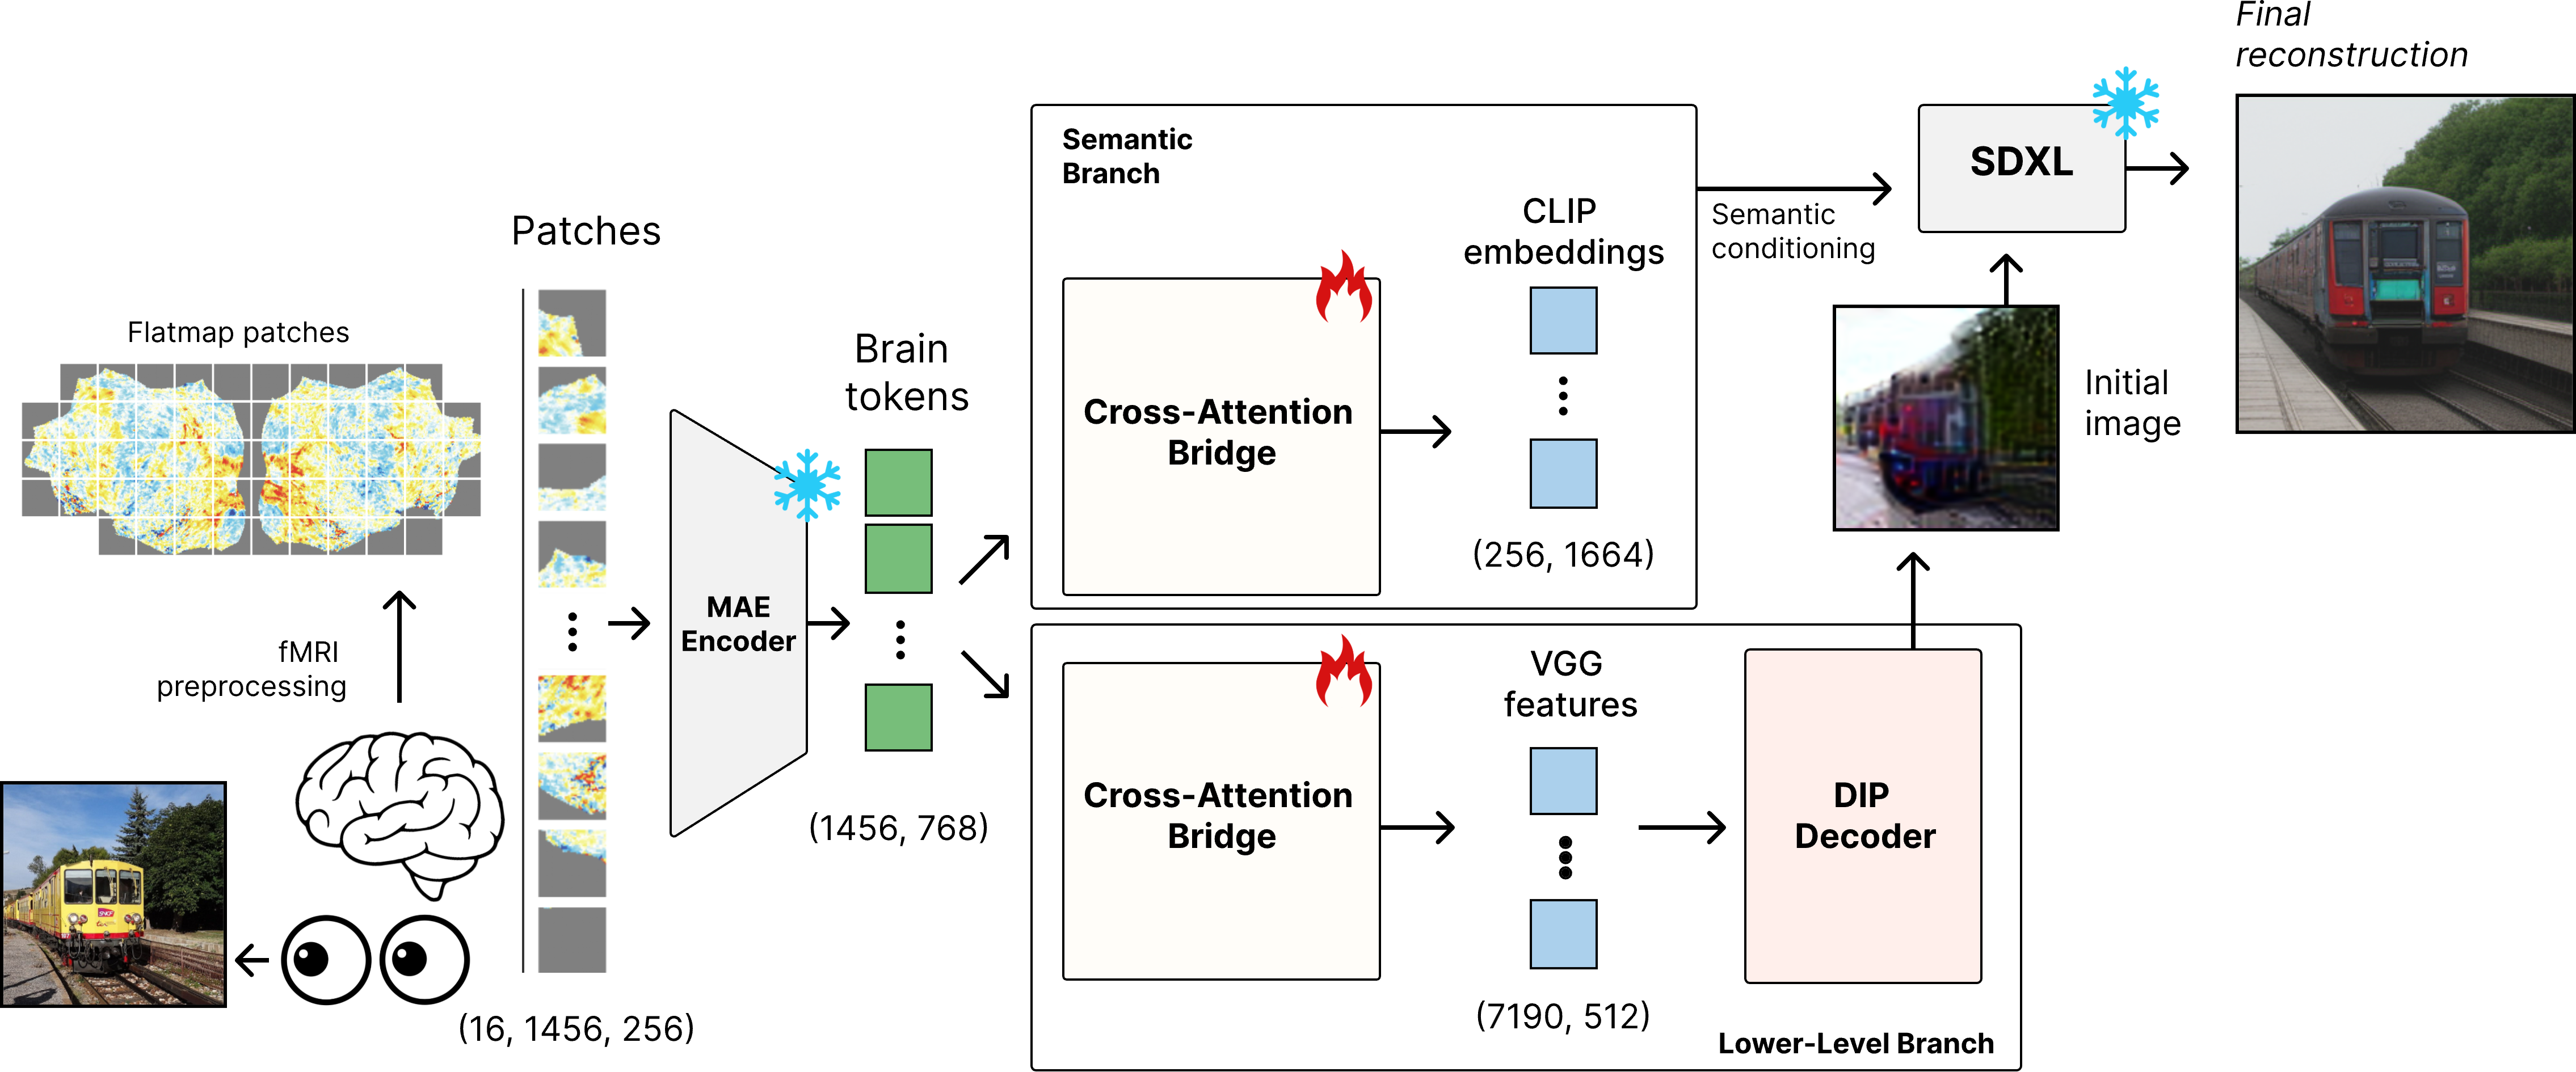
\includegraphics[width=0.75\textwidth]{images/model4.png}
\caption{CortexDecoder overall schematic. From the left side, single-trial betas are projected into 2D cortical flatmaps, then divided into patches. The patches are then encoded by the frozen CortexMAE encoder into 1456 brain tokens, each token having 768 dimensions. The cross-attention bridges, the only trained components, map these tokens into two representation, one for each branch. The semantic branch predicts 256 unpooled OpenCLIP ViT-bigG/14 tokens used as conditioning for a frozen SDXL-unCLIP \cite{ramesh2022hierarchicaltextconditionalimagegeneration} decoder. The lower-level branch predicts 7190 VGG16-BN feature tokens, which a Deep Image Prior \cite{Ulyanov_2020} decoder inverts into an initial image which encodes for layout, structure of objects and color. Finally a SDXL-unCLIP model takes the initial image and semantic embedding for conditioning to generate the final reconstructed image. Images including those depicting faces are derived from the Microsoft COCO dataset, used under CC-BY 4.0. \cite{lin2015microsoftcococommonobjects}}
\label{fig:model_schematic}
\end{figure*}
